\documentclass[11pt, oneside]{article}   	% use "amsart" instead of "article" for AMSLaTeX format
\usepackage{geometry}                		% See geometry.pdf to learn the layout options. There are lots.
\geometry{a4paper}                   		% ... or a4paper or a5paper or ... 
%\geometry{landscape}                		% Activate for for rotated page geometry
%\usepackage[parfill]{parskip}    		% Activate to begin paragraphs with an empty line rather than an indent
\usepackage{graphicx}				% Use pdf, png, jpg, or eps§ with pdflatex; use eps in DVI mode
\usepackage{array}							% TeX will automatically convert eps --> pdf in pdflatex		
\usepackage{amssymb}
\usepackage{cite}
\usepackage[draft]{fixme}
\usepackage{pdfpages}

\parskip 6pt % 1pt = 0.351 mm
\parindent 0pt

\title{Requirement Engineering Process in AMIDST}
\author{The handsome AMIDST guys et. al.}
\date{Latest version, \today}							% Activate to display a given date or no date

\begin{document}
\maketitle
%
%\begin{abstract}
%\end{abstract}
%

\section{Introduction}

Even though the number of algorithms designed for learning on streaming data is increasing, there is still not a unified and well accepted way for evaluating them.  This is because testing and evaluating algorithms that are designed to work on streaming data are more difficult those designed to work on static data.  There are both statistical and computational reasons for this.  

Static data is data, where each instance can be assumed to be identically and independently distributed i.i.d.  On streaming data, one can often not assume that data instances are i.i.d.  Moreover, the algorithms are often designed to weight measurements that are close to the actual time step higher than measurements that are further back.  On streaming data, we must therefore assume that data are generated from underlying distributions that are time dependent and also that the algorithms themselves are time dependent.  

Computational challenges are related to the fact that the data come from an open-ended data stream, conceptually infinitely long, which imposes practical challenges related to restrictions on cpu-time and memory allocation.  

Various error measures related to stream data has been proposed in the papers of Gama et. al. \cite{Gam09}, \cite{Gam09_2}, \cite{Gam12}.  A loss function is typically related to the penalty of misclassifications on classification problems or residuals in regression models.  The holdout error is basically the average loss on a holdout dataset of fixed size.  The predictive sequential, or \emph{prequential} error is defined as the average loss function up to time step $i$, where $i$ is the current time step.  Moreover, it was also suggested to use a prequental error measure, which involved a forgetting factor such as using a time window or fading factors.  In paper \cite{Gam12}, convergence towards the Bayes error was shown for all these performance measures provided that the learners are consistent and data are i.i.d.  Moreover, it was shown that if data was allowed to drift over time, meaning that samples are only locally i.i.d, then the prequental error measures with forgetting mechanisms were favourable.

\todo{Relate to other work on streaming data as well.}

The applications that are covered in this report have different characteristics than the applications discussed in \cite{Gam12}.  Some problem will be evaluated on a holdout dataset assuming i.i.d and a stationary algorithm.  Other problems can not assume i.i.d on a local scale, but stationarity can be assumed on a larger time scale.  

In this paper we will establish formal procedures for testing and evaluating the developed models and algorithms. This includes specification what metrics are relevant to use to quantify the ability of the AMIDST system, such as relevant formalization of loss functions, maximum response-times, memory limits and output format.  The paper will also include 
considerations about what quantitative improvements AMIDST should obtain over state of the art.

In section \ref{sec:methodology}, AMIDST relevant methodologies for evaluation of both batch and streaming algorithms are identified and discussed.  This section forms the foundation of the subsequent sections, where the exact evaluation routines for each use case provider is given. These sections contains a description of the requirements related to evaluation as described in Delivery 1.2, a short description of the algorithms and the data and finally methods for evaluating predictive and runtime performances.  Section \ref{sec:conclusion} concludes the report.


%\quote{\emph{Task description: In this task we will establish formal procedures for testing and evaluating the
%    developed models and algorithms. This includes specification of maximum response-times, output format,
%    relevant formalization of loss functions, investigations into what metrics are relevant to use to quantify
%    the ability of the AMIDST system, and considerations about what quantitative improvements AMIDST should
%    obtain over state of the art.}}
%
%
%From Helge's slides at the WP 3 kickoff meeting:
%\begin{itemize}
%\item Massive datasets: find relevant techniques, ensure scalability, etc.
%\item Online evaluation of streams: find relevant techniques, ensure scalability, define behavior in changing environment, etc.
%\item Significance of results, e.g., considering changing environment vs. ``reproducability'', distribution for test-statistic, significance levels/sizes of test-sets, etc.
%\end{itemize}


\section{Basic principles in requirement engineering}
\label{sec:stateOfArt}

In practice, the requirement engineering process ends with a document containing a list with requirements, which are in the form of what a software must do or comply with.  

To date there is no common definition of requirement engineering.  Some definitions focus on elicitation of requirements and therefore the interaction with the user, while others focus on the documentation or the specification.  A definition that takes both focuses into account is the IEEE standard given in \cite{Iee90}:

\emph{
\begin{enumerate}
\item The process of studying user needs to arrive at a definition of system, hardware or software requirements.
\item The process of studying and refining system, hardware or software requirements.
\end{enumerate}
}

In the context of understanding the requirement engineering process, it is worth spending some space on defining the requirement itself.  A definition of a requirement is given in IEEE standard \cite{Iee90}: 
\emph{
\begin{enumerate}
\item A condition or capability needed by a user to solve a problem or achieve an objective. 
\item A condition or capability that must be met or possessed by a system or system component to satisfy a contract, standard, specification or other formally imposed document. 
\item A documented representation of a condition or capability as in 1 or 2.
\end{enumerate}
}

This definition has a clear focus on the user, the system/system component and also which contract, standard or specification is needed to be met. Notice, that the requirement is related to \emph{what} a system can do and not \emph{how} it is done.

\subsection{Activities involved in requirement engineering}

The activities involved in requirements engineering vary widely, depending on the type of system being developed and the specific practices of the organization(s) involved  \cite{Som11}.  These may include:
\begin{itemize}
\item Requirements inception or requirements elicitation 
\item Requirements identification - identifying new requirements
\item Requirements analysis and negotiation - checking requirements and resolving stakeholder conflicts
\item Requirements specification (Software Requirements Specification) - documenting the requirements in a requirements document
\item System modeling - deriving models of the system, often using a notation such as the Unified Modeling Language
\item Requirements validation - checking that the documented requirements and models are consistent and meet stakeholder needs
\item Requirements management - managing changes to the requirements as the system is developed and put into use
\end{itemize}

These activities are sometimes presented as chronological stages although, in practice, there is considerable interleaving between them.  

\subsection{Use case driven requirement engineering}

It has always been a challenge for the software industry to communicate functionality to the users of a software. Moreover, software engineers are often frustrated, because users often do not know what they want. They only have an idea of what they want.  To improve this communication, the use-case driven approach was developed in the nineties.  It was first published by Ivar Jacobsen \cite{Jac92} and more modern references are \cite{Poh10} and \cite{Coc01}.  A use case focuses only on the interaction between a user and the system.  Requirements are always associated with a use case. This means that the user is requested to only focus on what he/she wants.  This is an advantage, compared to the traditional way where requirements are listed in relation to components and subcomponents in the software.  The traditional way often lead to a complexity that the user do not understand.  Also, it is more common with requirement duplicates in the traditional approach.

A use case is a list of steps, typically defining interactions between an actor and a system, to achieve a goal. The actor can be a human or an external system.  An overview on how to write effective use cases is given in \cite{Coc01}, where several templates are given. The use case providers are asked to provide the use cases in natural language and for each use case the following questions are central:

\begin{enumerate}
\item Who are the actors involved in the use case? An actor is either a person or an entity that interacts with the software.  
\item What is the main event that initiates the use case? This could e.g. be an external business event or a system event that causes the use case to begin.  It could also be the initial step in a normal work flow. 
\item What are the main user actions and system responses that will take place during the normal execution of the use case?. This dialog sequence will ultimately lead to accomplishing the goal that is implied by the use case name and description.
\item How can we evaluate the success of the use case?
\end{enumerate}
 
It is also common to group the users, or human actors, within an organization into a small set of user groups. The users within each user group need to have similar roles within their organization and their set of competences are expected to be similar. 

To understand the use case driven approach to requirement engineering better, it is useful to distinguish between functional and non functional requirements.  Functional requirements are those requirements that are directly related to the interaction between the user and the system.  The non functional requirements are more hidden for the user are related to the global overall success.  For instance scalability, traceability and testability.  When use cases are provided and functional requirements are identified, it is the requirement engineers role to identify, document and communicate these non functional requirements as well.  The use case driven approach to requirement engineering focuses on revealing the functional requirements together with the users.  This improves the communication between the users and the developers, because the focus is on what the users wants and less on how it can be done.


\section{The AMIDST requirements engineering process}
\label{sec:AmidstRequirementProcess}

This section contains a description of the AMIDST RE process.  We first describe the main characteristics of the AMIDST project that
influence and shape the requirements engineering process. Based on the these characteristics we describe the
AMIDST requirements engineering process that is based on the RE process \cite{} described in
Section~\ref{sec:stateOfArt} and tailored to the specifics of AMIDST. The focus of the requirements engineering process
is on the functionality and documentation of the software products being developed, and will, e.g., not cover process-related requirements.




%Prior to project start, the importance of requirement engineering was well acknowledged by the partners in the project.  This is evident from the %fact that 23 out of 310 person months were assigned to conduct the requirement analysis.  We have chosen to summarize the characteristics in t%he next subsections, which makes it is easier to refer to them later in this report.

\subsection{Characteristics of the AMIDST project}
\label{sec:characteristics}

In this section we identify and describe the key characteristics of the AMIDST project that directly influence the requirements
engineering process. 

%In this subsection, we list the main aspects or characteristics of the project that have the greatest impact on the design of the RE process.  Notice, that there are also many other characteristics of AMIDST that are not mentioned here.  This is because their impact on the RE process is believed to be minimal.  
%It is also worth noting that other researchers and practitioners that want to follow our path of describing characteristics of the project, may benefit from our analyses of which characteristics had the most impact on the RE process.

\ \\
\noindent \emph{Characteristics one:  Pre-specified scope of the project}
\label{sec:characteristic1}

The AMIDST project is funded by the European Union's Seventh Framework Programme for research, technological
development, and demonstration. The overall scope and main developments in the project are therefore defined from the
beginning of the project period and documented in the description of work \cite{}. This will henceforth be referred to
as the DoW framework. More detailed requirements pertaining
to the functionality and documentation of the developed software should thus fit within the DoW framework, and their
necessity in relation to AMIDST should be justified and demonstrated.   


 

% When the AMIDST project started, there was a document of work that was already agreed upon.  In particular the RE process must comply with this document and the software must comply with the deliveries in the work package one to eight.  In practice, this means that whenever a requirement is considered, it must always be justified and linked with a delivery in a work package.

\ \\
\noindent \emph{Characteristics two: Several partners at different geographical locations}
\label{sec:characteristic2}

The AMIDST consortium consists of 7 partners/stakeholders, 4 industrial and 3 universities, which are situated in 4 different
countries. The direct requirements engineering implications of this diverse consortium composition is twofold. 

First of
all, although AMIDST targets the industrial stakeholders' common need for processing massive data streams, the more
intrinsic aspects of the three industrial domains differ significantly. This, in turn, means that partners will have different
(possibly conflicting) requirements for the system being developed. To ensure that the requirements are comparable
across domains and abide to the DoW, a unified formal framework for eliciting system requirements is needed. Such a
framework may also provide transparency in the overall requirement engineering process and help prioritize requirements
across different domains and thereby help resolve possible conflicts.   

Secondly, with the project partners located in different countries, there is a need for a controlled and stringent requirements
process in order to limit the travel expenditures. This approach is supported by a unified formal requirements
engineering framework. Consultancy and discussions in relation to the
requirements will primarily be achieved through telecommunication conferences, and only secondarily by physical meetings. 
 
% The result is a project with many stakeholders, which have different backgrounds, priorities and influences on the software. Moreover, the partners are located in different countries, which implies that the financial and time costs for personal meetings are quite high.  This characteristic has an influence on the pursued RE process, because the process is restricted to not rely heavily on meetings with many participants.

\ \\
\noindent \emph{Characteristics three: Transference of domain knowledge between  partners}
\label{sec:characteristic3}

The industrial partners of the AMIDST project come from very different domains: the automotive, energy, and finance
industry. To support the development, refinement, and completion of the of unified formal requirements framework it is
necessary with a regular and structured communications among the project partners during the requirements engineering
process. 

% On one side, it was essential that the industrial partners gained enough insight of what can be done with
% probabilistic graphical models to identify proper use cases.  On the other side, it was essential that the academic
% partners gained enough knowledge about the industrial domains to understand the proposed use cases and requirements. 
%This was considered in the way we divided our work among the academic partners. 

\ \\
\noindent \emph{Characteristics four:  One framework for three different problems}
\label{sec:characteristic4}

The AMIDST system should define a general framework that can encompass the diverse domains of the three industrial
partners. This puts constraints on the format of the unified formal requirements framework as it should be sufficiently general to
allow for all relevant requirements to be elicited for the three domains. Furthermore, to allow for a controlled and
balanced system development, the specification of the requirements should be consistent across domains and be linked to
relevant project phases, work packages, and tasks. The latter, in particular, will provide the work package leaders with
a clear overview of the requirements that are relevant for the activities in a specific work package.   

%One single framework shall solve all posed problems.  It is therefore a challenge to find common requirements that are addressing problems across all three domains.

\ \\
\noindent \emph{Characteristics five: Potential refinement of project focus}
\label{sec:characteristic5}

AMIDST is a research project, where both the industrial and academic partners' understanding of the domains develop as
the project unfolds. In order to support a potential refinement of the project's focus and goals, the requirements
engineering process should allow for an internal (re)prioritization of the requirements that is transparent across
application domains.    


% The posed problems are challenging and, as usual, some aspects of the problems are not fully understood at this stage in the project. We realize that the priority of some of the requirements can change as the project continue. There is also an uncertainty related to how satisfied the industrial partners will be when the proposed solutions are implemented.  

%Defining a requirement is linked with the perception of which design pattern to follow \cite{Ral13}.  A design pattern is chosen by the software %developer and is basically the path to meet the requirement.  As explained in \cite{Ral13}, when there is a high degree of unclarity of which  design %pattern to follow, this ambiguity is transferred to the definition of the requirement as well.  The goal of the AMIDST software is to reach targets %that are highly innovational, meaning that it is particularly difficult to define requirements that are clear and unambiguous.


\subsection{Project phases and AMIDST requirements identification }

%% We decompose the overall project period into phases to better -> support identification of requirements and work
%% package allocation.


In order for a requirement to be useful for the software engineers, they are often associated with steps in a product life cycle as for instance described in \cite{Eig09}.  In this reference the overall life cycle is divided into three phases; design phase, operation phase and disposal phase.  In the AMIDST software, the disposal phase is not relevant for us.  This is shown in figure \ref{REprocess2}.

\begin{figure}[htbp]
\centering
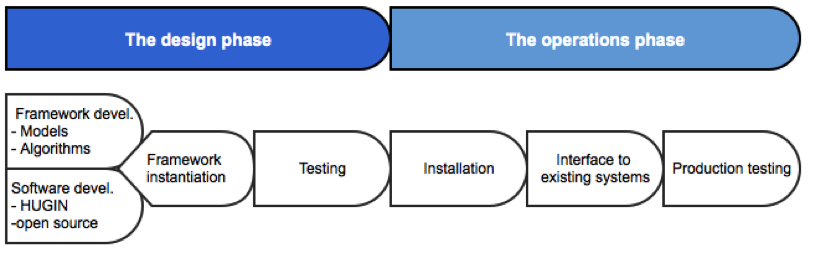
\includegraphics [keepaspectratio,width = 14cm] {REprocess2}
\caption{The table show key steps in the design and operation stages. Notice that each requirement can only be member of one step.} 
\label{REprocess2}
\end{figure}

The design stage contains general functionality requirements for the system, i.e. what the system should do and support.
In figure \ref{REprocess2}, we detail key steps inside this phase. The first step consists of the design of the general
framework (models and algorithms) as well as the design and development of the software tools. the phases are primarily
related to Work packages 1--5. In a second step, the general framework and software is instantiated for each specific use case. Finally, initial tests of the use case instantiated framework are conducted.  At the design phase, possible design requirements could e.g. address
\begin{itemize}
 \item the scope of the model
 \item the interpretability of the learned models
 \item the extent and type of domain knowledge that can be integrated into the models
 \item documentation
\end{itemize}

The requirements for the operation phase concern the functionality of the deployed system. In figure \ref{REprocess2}, we decompose this phase into three stages: installation, interface to existing systems, and production testing. The requirements for this phase could e.g. address
\begin{itemize}
 \item hardware constraints
 \item interfaces to existing software or data base systems
 \item inference functionality, i.e., what queries the system should be able to answer
\end{itemize}


\subsubsection{Use cases and user groups in the requirements engineering process}

A use case driven approach is chosen in the AMIDST RE process.  In a use case driven approach, there is a clear focus on the functional requirements which are the most relevant to the user.  It is also important that requirement are listed with respect to each use case, meaning that the users get a better overview than if requirements are listed component-wise. The use case driven approach is designed to ease the communication between the user and the software developer.  It is therefore a good choice to meet characteristic three.  

Moreover, since the functional requirements are generally more high-level, this approach comply with characteristic five.  This is because it is less likely to add a very specific requirement that becomes less relevant later.  

In order to meet characteristic one, the use case providers are asked to describe how every use case can be tested and what is needed for them to deem the product a success.  These requirements are identified as performance requirements.

\subsection{The general AMIDST requirements engineering process}
\label{sec:reprocess}

The activities in the requirement engineering process is carried out in an iterative fashion that is expected to involve a high level of cooperation and interaction between the partners in order to meet all characteristics in subsection \ref{sec:characteristics}. 

In figure \ref{REprocess1}, an illustration of the requirement engineering process for AMIDST is given, which is inspired by \cite{Ebe10}.  In general the process contain five phases, which are discussed below.
\begin{enumerate}
\item Preparation I.  This phase starts at the same time as work package one and ends when the initial template, attachment X1, for the requirement engineering document is finished.  In this template, the requirement engineering process is outlined including definitions of use cases, user groups and how to link requirements with stages in development process.  In order to meet characteristic three, four and five, the use case providers are asked to provide a detailed description of the system context that the AMIDST software is expected to run in, identify user groups, describe use cases and requirements.  In order to meet characteristic four, the requirements are linked with references to stages in the development cycle. 
\item Elicitation. The distribution of the above mentioned template marks the initialization of this phase.  Its aim is to get an initial high-level description of the different use cases and their requirements. This information are specified by the use case providers in collaboration with the academic partners to meet characteristic one, three and four.  Once the use case providers return the present document with the requested information, feedback and informal meetings are expected to clarify and refine the information provided.  At the end of the elicitation phase, the aim is to have a first coherent description of the requirements for each use case provider.
 \item Prioritization. In this phase the use case providers completes an extended version of the document template used in the previous phase. This template is used to link each of the requirements to the relevant work packages and tasks in the AMIDST project to meet characteristic one. Moreover, the template allows the use case providers to provide a more fine grained prioritization of the relevant requirements for the AMIDST framework.  Specifically, the use case providers are asked to rate each requirement in terms of must, should and could and also rate how important the requirement is to them.  
\item Validation. In this phase, the requirements from all use-case providers are collected to get the \emph{big picture}.  This involves a discussion to what extent the requirements can be accommodated. Revisions and negotiations of the detailed requirements are therefore expected.  In this phase, it is important to ensure that characteristic one is met.
 \item Evaluation and Testing. In this phase, the focus is on the elicitation of the evaluation and testing procedures in the AMIDST project. This phase starts with the distribution of a new document template, where the aim is to obtain a high level description of the evaluation and testing methods that is necessary to measure the performance of the AMIDST framework.
\end{enumerate}

\begin{figure}[htbp]
\centering
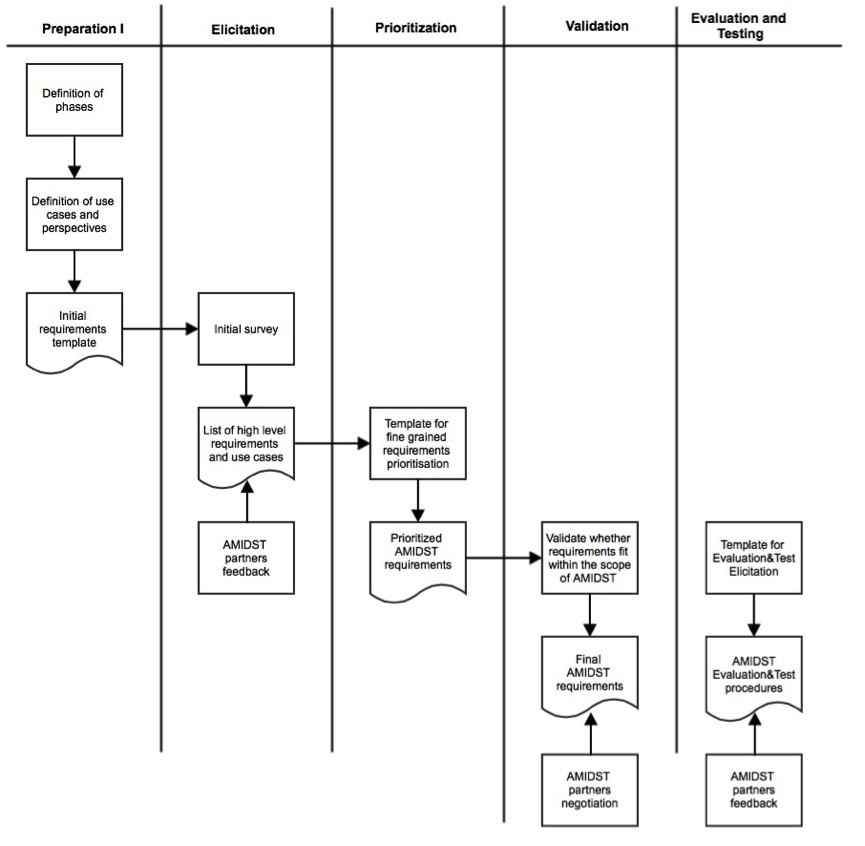
\includegraphics [keepaspectratio,width = 14cm] {REprocess1}
\caption{Description of the five phases in the requirement engineering process in AMIDST.}
\label{REprocess1}
\end{figure}



% \subsection{Main aspects of the AMIDST's RE process}
% \label{sec:reprocess}

% In this subsection, we detail the main elements that define the AMIDST RE process, which are strongly influenced by the characteristics in the previous subsection.  This subsection contains a description of how the work is divided among the partners and how the use case driven approach is adapted.  Moreover, a document template that is central in the AMIDST RE process is described.  Requirement are discussed in terms of how they are linked with the product life cycle and deliveries in the AMIDST project.  Prioritization of requirements are also briefly described, before the outline of the main activities in the AMIDST RE process is given.



%%% Local Variables: 
%%% mode: latex
%%% TeX-master: "REproccess"
%%% End: 



\section{Realization of the requirements engineering process}
\label{sec:realization}

The RE process was organized by coupling each use case provider with an
academic partner; Verdande Technology was paired with NTNU, DAIMLER was paired with AAU and Hugin, and CajaMar was paired with
UAL. The particular partner associations were based on geographical as well as affinity
considerations. It is important to stress that the RE process does \emph{not} prescribe such a
partner association, but it does bring distinct advantages. First of all, the academic partners can better assist the use case
providers when completing the requirements template, and the ongoing internal communications and discussions (both formal
and informal) provide an opportunity for early feedback on drafts of the requirements
specification. Secondly, this division of work also provides an increased knowledge transfer between industrial and academic
partners. 

% This part of the report is written in month six when most of the process is conducted.  This section contains a few points on what experiences we have gained in the project so far:

% \begin{enumerate}
% \item Everyone involved has had a learning experience on many levels.  The industrial partners have learned about probabilistic graphical models, while the academic partners have learned about the industrial domains.  Most participants have increased their knowledge on how to conduct a requirement analysis. 
% \item There has only been one meeting where all stakeholders have met, which was the kickoff meeting in Denmark in month three.  Most communication has been done through Skype and email, but also a few face to face meetings have taken place. Most of the communications have been related to clarifications in terms of filling out the template X1.
% \item There have been adjustments of the template X1 as the process has proceeded.  Examples of this is adding fields to the requirements so they could be linked to concrete tasks in the AMIDST project or adding columns for rating the importance of a requirement.
% \end{enumerate}



% \subsubsection*{Division of work}

% For each industrial partner, a mentor among the academic partners is assigned. The mentor for Verdande Technology is NTNU, the mentor for DAIMLER is AAU; and the mentor for CajaMar is UAL. Hugin has a coordination role. On one side, this allows each of the academic partners to focus on only one industrial domain.  On the other side, the industrial partners have the academic support they need for identifying proper use cases.  This division of work is a tool to mitigate characteristic two, because it eases the knowledge transfer between the industrial and academic partners. 


As described in Section~\ref{sec:AmidstRequirementProcess} one of the design considerations for the requirements
engineering process was to base the requirements specification on a formal template that would be shared by
all three use case providers. In addition to the information that the use case providers are requested to fill-in, the
template also provides a description of the overall RE process as well as guidelines on how to
complete the template. A generic template can be found in Appendix~\ref{sec:form-fram-requ}.

  
% Because of characteristics two, we have decided to not follow a RE process that heavily relies on personal meetings and
% direct personal interviews.  Even though meetings still is an important ingredient in the process, we decided to
% distribute a document template to each of the industrial partners early in the process. 

The completion of the templates was conducted as an iterative process with a close collaboration between the use case
providers and the paired academic partners. In addition to the more formal deadlines marking transitions between 
phases in the RE process, we also introduced several short-term deadlines, where
the use case providers were given feed-back on draft versions of their completed templates. Not only did this serve as an
instrument to ensure a continuous progression in the requirements specification, where misunderstandings and problems
could be identified and mitigated at an early stage, but it also provided an early transfer of knowledge from the
industrial partners to the academic partners in the project. Part of this (otherwise tacit) knowledge were documented
for the benefit of the other partners, both current and future, in the consortium, and is expected to be included 
in the deliverables planned for Work packages 6--8. This, e.g., includes a description of the data characteristics for
the use case providers. 

% \begin{itemize}
% \item Industrial partners are pushed to contribute with use cases early, meaning that issues and misunderstandings are revealed early.  This is important to mitigate characteristic three.
% \item All ideas are documented and there is no loss of information, which is common in interviews.  This is important to meet characteristic one, three, four and five.
% \item The provided information can easily be transferred from the mentors to the other academic partners.  This is important for meeting characteristic four.
% \item  The partners can spend more time on use cases and requirements, before talking to the mentors.  To some extent, this meets characteristics three, because it is easier for the mentors to learn when the requirements are more though through.
% \item The work on the different templates can be asynchronous in time.  This eases the resources allocation for the different partners.  This is related to characteristic two.
% \end{itemize}

The specified requirements (identified by a unique label as described in Appendix~\ref{sec:form-fram-requ}) together
with their work package/task allocations and prioritizations will be summarized in
tables at the work package level. These tables allow work package leaders to get a clear overview of the specific
requirements that need to be taken into account in the different work packages. An example of a part of such a work
package requirements table can be found
in Table~\ref{tab:WP2-requirements}, which includes some of the presently collected requirements pertaining to Work package 2. 


\begin{table}[htbp]
  \centering
  \begin{tabular}{|c|c|c|c|c|}
    \hline
    Req.\ ID.\ & Relevant subphase & Must/should/could & Points & Task \\ \hline\hline
    DAI.U5.D1 & Framework devel.\ \& instan.\ & Should & 20 & 2.2  \\
    DAI.U5.D2 & Framework devel.\ \& instan.\ & Should & 20 & 2.2  \\
    DAI.U5.D3 & Framework devel.\ & Should & 15 & 2.2  \\
    DAI.U5.D4 & Framework devel.\ & Should & 15 & 2.2  \\
    DAI.U5.D4 & Framework instant.\ & Should & 20 & 2.2  \\
    DAI.U7.D1 & Framework devel.\ & Must & 35 & 2.1 \\
   \vdots & \vdots  & \vdots & \vdots & \vdots \\ \hline\hline
  \end{tabular}
  
  \caption{The work package requirements table containing the presently collected requirements for Work package 2.}
  \label{tab:WP2-requirements}
\end{table}



%%% Local Variables: 
%%% mode: latex
%%% TeX-master: "REproccess"
%%% End: 


\section{Conclusion, observations and reflections} \fixme{For a
  possible publication, we could report on our (including the use case providers') experiences with the process, but
  since we are not yet finish with the RE process there is not that much to report \ldots }
\label{sec:conclusion}

This document describes the requirement engineering process pursued in AMIDST. The general process is  adapted and based
on previously described approaches to requirements engineering, but tailored to the specific needs and characteristics of the AMIDST
project. In particular, the idiosyncratic aspects of the AMIDST project that combined distinguishes it from other software
projects at the requirements engineering level, include (i) a pre-defined project scope, (ii) many different
stakeholders, and (iii) the development of a sufficiently general software framework that can be instantiated for
use case providers representing different industries.  Central to the requirements engineering approach is the use case
concept that forms the basis for the requirements specification. The actual specification is document in a generic
formal template that allows for the elicited requirements to be compared and prioritized across domains. 

The division of work realized in the AMIDST project was partly successful due to the natural coupling (geographical and
affinity based) between the industrial partners and the academic partners. This type of work division may not be
achievable in projects with a larger number of partners or where the partners are not geographical co-located. On the
other hand, it should also be emphasized that this division of work is \emph{not} as such prescribed by the proposed
requirements engineering process. 


\bibliographystyle{splncs}
\bibliography{re}

\appendix


\section{Formal framework for requirements elicitation}
\label{sec:form-fram-requ}
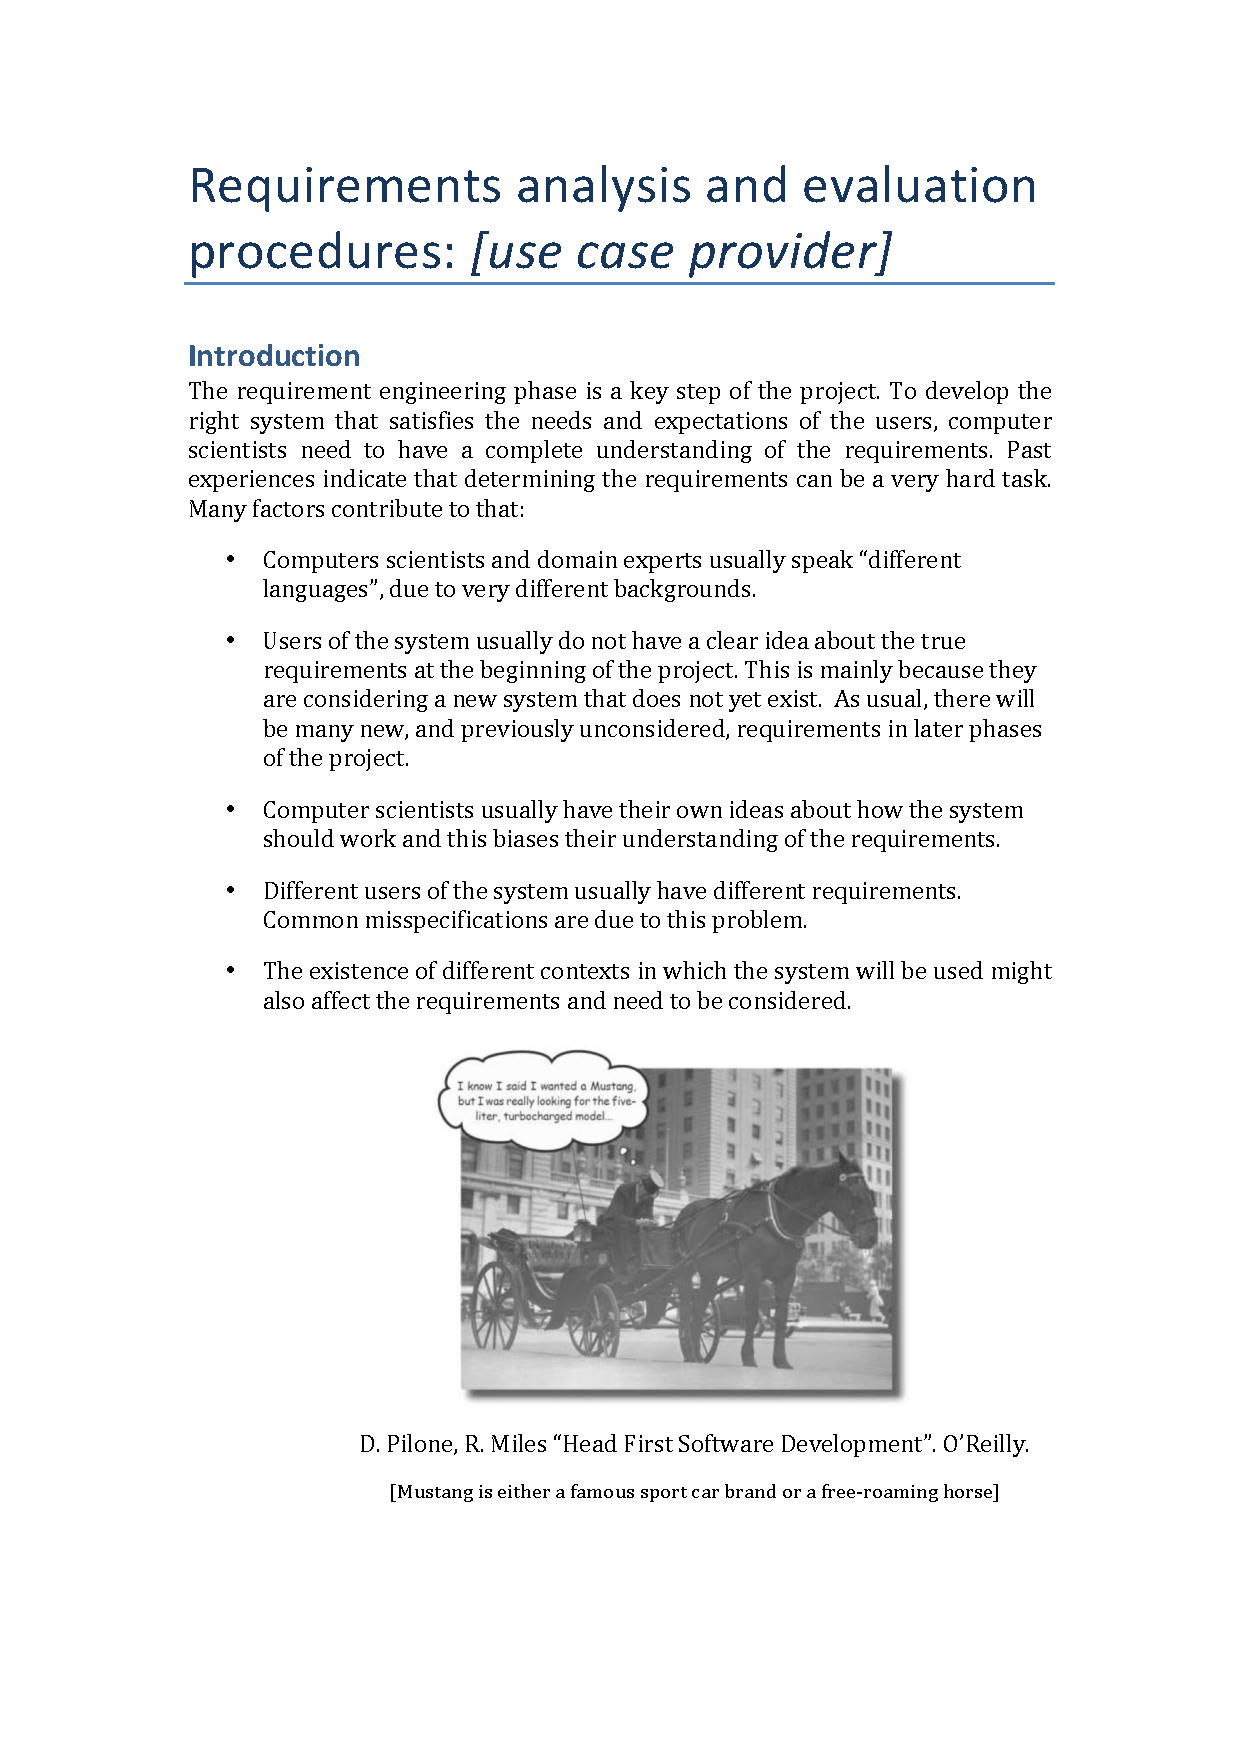
\includepdf[pages={-}]{appendixA1.pdf}
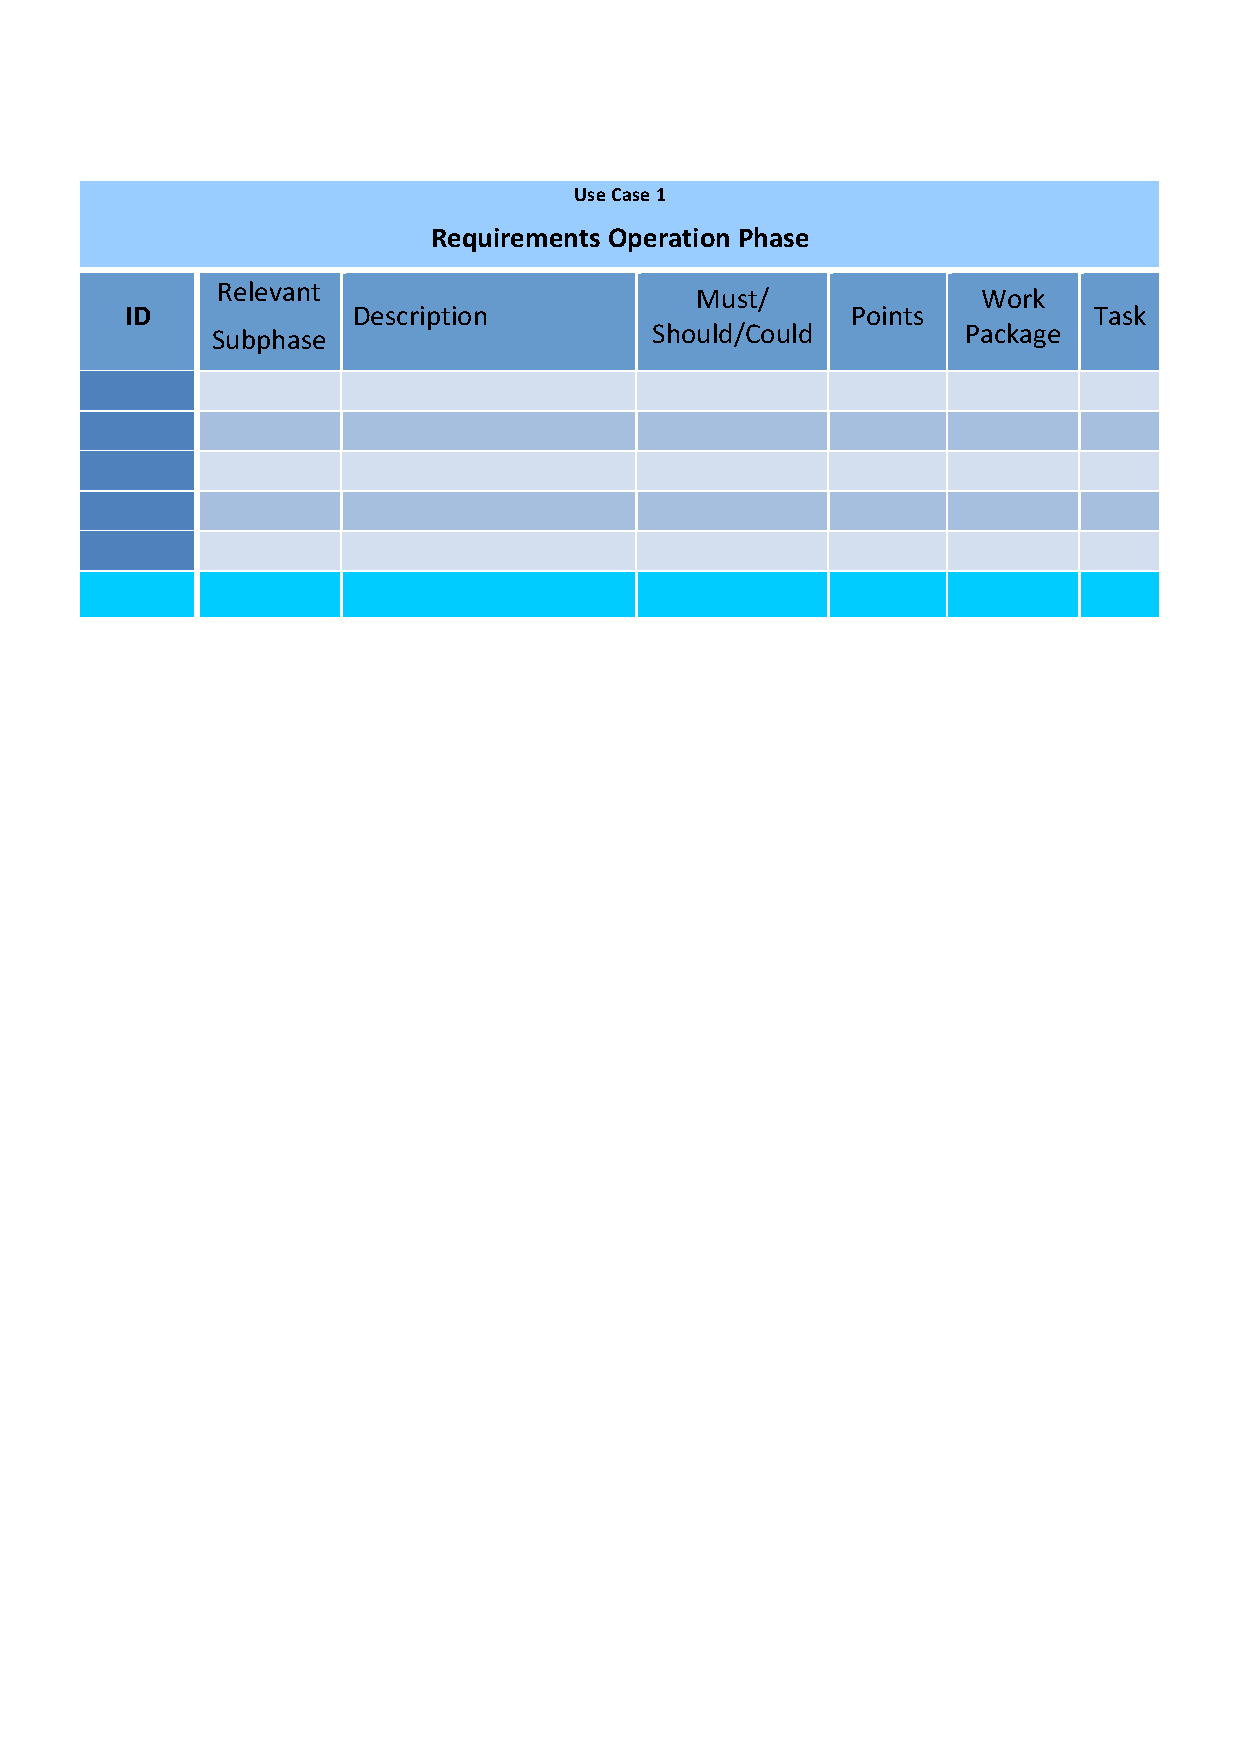
\includepdf[pages={-}]{appendixA2.pdf}

\end{document}  